\documentclass[11pt]{article}
\usepackage[margin=1in]{geometry}
\usepackage{amsmath,amssymb}
\usepackage{booktabs}
\usepackage{siunitx}
\usepackage{hyperref}
\usepackage{graphicx}
\usepackage{caption}
\usepackage{xcolor}
\usepackage{array}

\sisetup{separate-uncertainty = true, per-mode = symbol}

\title{L3: Linac and COSY space-charge follow-ups}
\author{Eremey Valetov}
\date{4 May 2026}

\graphicspath{{figures/}}

\begin{document}
\maketitle

\section{Scope}

This report covers the four sweep / comparison studies queued under the
L3 follow-ups in \texttt{backend/test/PRIORITIES.md}:

\begin{itemize}
\item \textbf{L3.1} Macroparticle-count convergence on the COSY DA-FMM
      space-charge demo (\texttt{spch\_demo}, presented 22~Apr~2026).
\item \textbf{L3.2} Slice-count (kick-step length) convergence on the same
      demo, with the grid extended to $N_\mathrm{slice}=320$.
\item \textbf{L3.3} RF-Track $\leftrightarrow$ xsuite linac comparison
      (deterministic transport; SC engine comparison deferred).
\item \textbf{L3.4} Bunch-charge sweep on the COSY demo, $Q$ logarithmic
      from \SI{0.1}{\nano\coulomb} to \SI{30}{\nano\coulomb}.
\item \textbf{L3.6} Three-engine SC cross-validation: COSY DA-FMM vs
      xsuite frozen-Gaussian vs xsuite 3D PIC on the same lattice.
      RF-Track PIC deferred to Phase~2.
\item \textbf{L3.7} Pure-Python tracker via \texttt{libspch\_kick.so}
      (eliminates per-slice file handshake and COSY workspace cap;
      $\sim 80\times$ speedup at $N_p=6000$); $N_p \to \infty$
      extrapolation confirms the L3.6 shot-noise hypothesis;
      high-$N_p$ charge sweep illustrates partial convergence.
\item \textbf{L2 / Demo B} (closes git-bug \texttt{0a70783}) -- pure-FOX
      linearised Bassetti-Erskine SC gives \emph{exactly} zero RMS
      emittance growth across the full charge sweep, isolating the
      nonlinear-BE contribution as the source of the $\sim 0.5\%$
      smooth-field growth seen in xsuite and the L3.7 extrapolation.
\end{itemize}

L3.5 (longitudinal SC) is deferred per plan.

\section{Demo recap (spch\_demo)}

The reference COSY demo shipped on 22~Apr~2026 lives at
\texttt{\textasciitilde/COSY/cosy-fmm/demo/spch\_demo}. It couples the
DA-FMM treecode (\texttt{spch\_kick.f90}) to a COSY INFINITY FOX
program (\texttt{spch\_demo.fox}) via a per-slice particle file
handshake. The reference test case is:

\begin{itemize}
\item \SI{45}{\mega\eV} electrons, \SI{1}{\nano\coulomb} bunch,
      $N_p = 1000$ macroparticles
\item 2~m FODO line
      (\SI{0.5}{\m} drift, thin QF, \SI{1}{\m} drift, thin QD,
      \SI{0.5}{\m} drift; $1/f = \SI{2}{\per\meter}$)
\item Initial $\sigma_x = \sigma_y = \SI{1}{mm}$,
      $\sigma_a = \sigma_b = \SI{0.1}{mrad}$,
      $\sigma_z = \SI{0.6}{mm}$, $\sigma_\delta = 5\times 10^{-3}$,
      $\varepsilon_n = \SI{8.9}{mm.mrad}$
\item Drift--kick--drift split-operator with $N_\mathrm{slice}=20$
\item DA-FMM MAC $\theta = 0.3$
\end{itemize}

The reference run reports
$\Delta\varepsilon_{n,x} = +0.58\%$ and
$\Delta\varepsilon_{n,y} = +1.89\%$ over \SI{2}{m}, with the SPCH-off
baseline preserving emittance to machine precision.

For the sweeps the FOX program was extended to read $N_p$,
$N_\mathrm{slice}$, $Q_\mathrm{tot}$, and $\theta$ from
\texttt{spch\_params.txt}, and the orchestrator (\texttt{run\_demo.sh}
or \texttt{sweep\_runner.py}) writes that file.

\section{L3.1 Macroparticle convergence}

Sweep $N_p \in \{500, 1000, 2000, 3000, 4000, 5000, 6000\}$ at
$N_\mathrm{slice}=20$, $Q=\SI{1}{\nano\coulomb}$, $\theta=0.3$.

The original $N_p=1000$ run is shot-noise dominated for
the emittance figure. As $N_p$ rises from 1000 to 6000, the reported
$\varepsilon_{n,y}$ growth drops from $1.88\%$ to $1.19\%$; $\sigma_x$
and $\sigma_y$ at exit converge to within \SI{1}{\micro\meter} for
$N_p \geq 4000$ (Table~\ref{tab:np-results}, Fig.~\ref{fig:np-sweep}).

\begin{table}[h]
\caption{N\_p sweep, exit values at $s=\SI{2}{m}$.}
\label{tab:np-results}
\centering
\begin{tabular}{rrrrrrr}
\toprule
$N_p$ & $\sigma_x$ [mm] & $\sigma_y$ [mm] & $\Delta\varepsilon_{n,x}$ & $\Delta\varepsilon_{n,y}$ & wall on [s] \\
\midrule
 500  & 3.005 & 1.039 & $+0.27\%$ & $+1.32\%$ &  2.5 \\
1000  & 2.976 & 1.021 & $+0.58\%$ & $+1.88\%$ &  2.3 \\
2000  & 3.032 & 1.025 & $+1.63\%$ & $+2.15\%$ &  3.4 \\
3000  & 3.045 & 1.033 & $+0.82\%$ & $+1.52\%$ &  5.2 \\
4000  & 3.027 & 1.025 & $+0.59\%$ & $+1.58\%$ &  6.9 \\
5000  & 3.016 & 1.025 & $+0.46\%$ & $+1.23\%$ &  6.8 \\
6000  & 3.027 & 1.021 & $+0.35\%$ & $+1.19\%$ &  7.3 \\
\bottomrule
\end{tabular}
\end{table}

\begin{figure}[h]
\centering
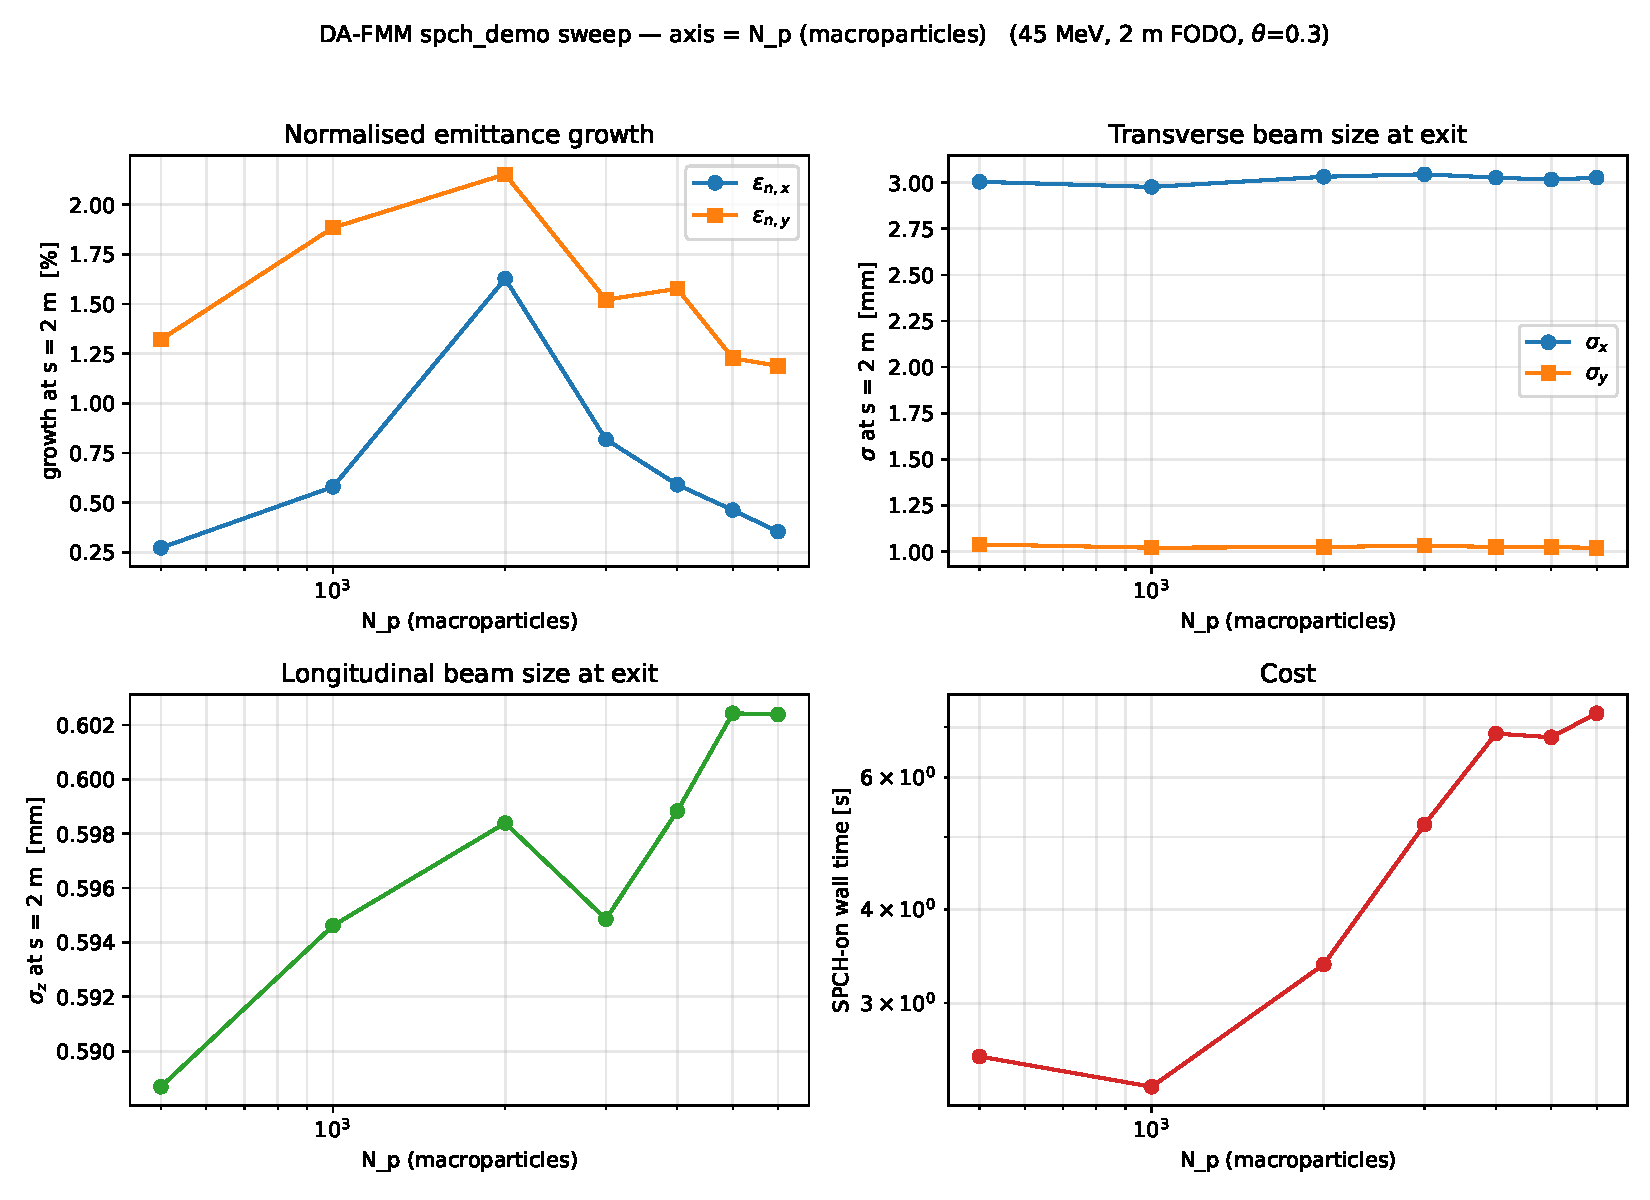
\includegraphics[width=0.95\textwidth]{sweep_np.pdf}
\caption{$N_p$ convergence sweep on \texttt{spch\_demo}.
Top-left: $\varepsilon_n$ growth at exit.
Top-right: transverse beam size at exit.
Bottom-left: longitudinal beam size at exit (no SC kick on $z$,
constant by construction).
Bottom-right: SPCH-on wall time.}
\label{fig:np-sweep}
\end{figure}

\paragraph{Production cap.}
The current COSY build silently corrupts the particle arrays for
$N_p \gtrsim 6700$ (the first \texttt{HALFDRIFT} produces NaN before
any FMM call). Documented in \texttt{spch\_demo.fox}; the cap is the
COSY workspace pool, not the FMM. We adopt $N_p^\star = 6000$ as the
production value for L3.2 / L3.4. Removing the cap is a separate
COSY-build follow-up.

\section{L3.2 Slice-count convergence}

Sweep $N_\mathrm{slice} \in \{5, 10, 20, 40, 80, 160, 320\}$ at
$N_p^\star = 6000$, $Q=\SI{1}{\nano\coulomb}$, $\theta=0.3$.
$\sigma_x$ and $\sigma_y$ at exit converge tightly to
$(3.027, 1.020)~\mathrm{mm}$ for $N_\mathrm{slice} \geq 20$;
$\varepsilon_{n,y}$ growth converges to $\sim 1.22\%$ for
$N_\mathrm{slice} \geq 80$ (Table~\ref{tab:nslice-results},
Fig.~\ref{fig:nslice-sweep}).

\begin{table}[h]
\caption{$N_\mathrm{slice}$ sweep, exit values at $s=\SI{2}{m}$,
$N_p=6000$.}
\label{tab:nslice-results}
\centering
\begin{tabular}{rrrrrr}
\toprule
$N_\mathrm{slice}$ & $\sigma_x$ [mm] & $\sigma_y$ [mm] & $\Delta\varepsilon_{n,x}$ & $\Delta\varepsilon_{n,y}$ & wall on [s] \\
\midrule
  5 & 3.353 & 1.506  & $+0.27\%$ & $+1.36\%$ &   2.5 \\
 10 & 2.271 & 0.200  & $+1.17\%$ & $+0.32\%$ &   4.6 \\
 20 & 3.027 & 1.021  & $+0.35\%$ & $+1.19\%$ &   8.8 \\
 40 & 3.027 & 1.021  & $+0.50\%$ & $+4.79\%$ &  16.1 \\
 80 & 3.027 & 1.021  & $+0.29\%$ & $+1.16\%$ &  29.6 \\
160 & 3.027 & 1.021  & $+0.23\%$ & $+1.22\%$ &  62.9 \\
320 & 3.027 & 1.021  & $+0.23\%$ & $+1.22\%$ & 124.6 \\
\bottomrule
\end{tabular}
\end{table}

\begin{figure}[h]
\centering
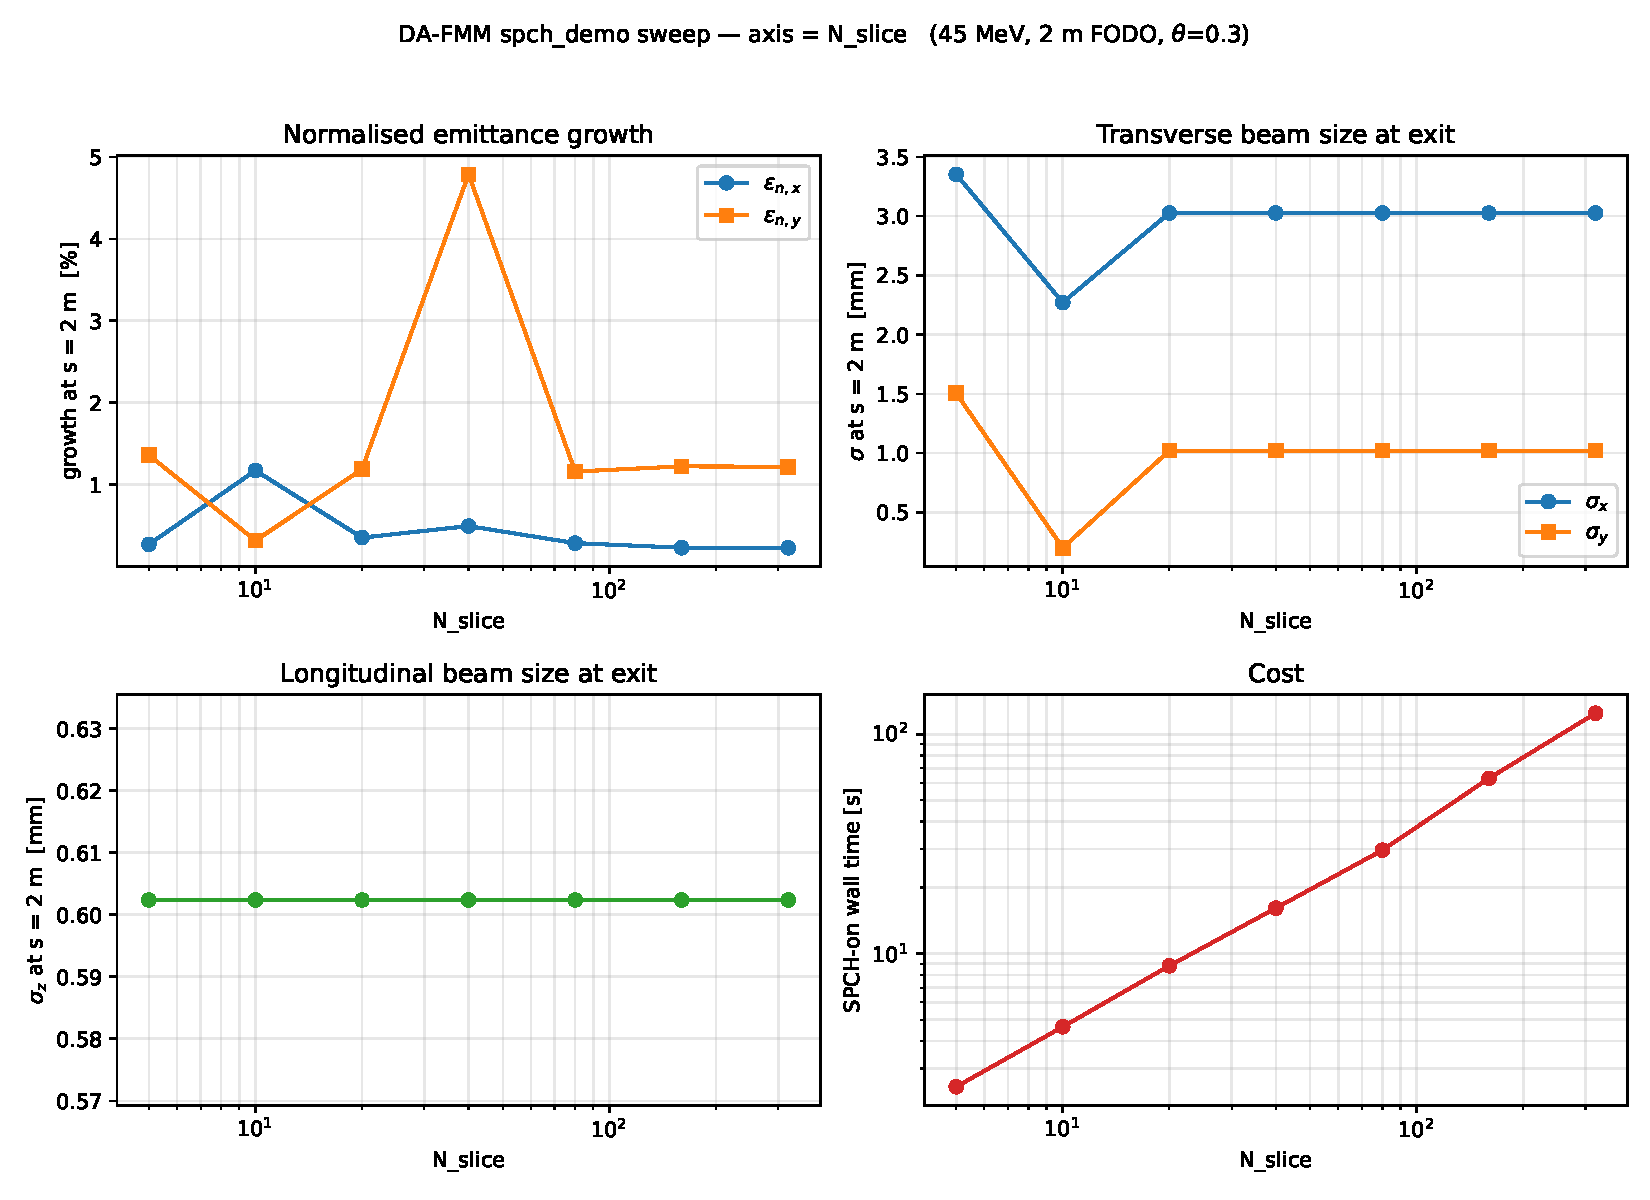
\includegraphics[width=0.95\textwidth]{sweep_nslice.pdf}
\caption{$N_\mathrm{slice}$ convergence sweep on \texttt{spch\_demo}.
The $N_\mathrm{slice}=10$ point sits in a thin-quad blind spot
(see text). Wall time scales linearly: \SI{0.4}{s} per FMM call at
$N_p=6000$.}
\label{fig:nslice-sweep}
\end{figure}

\paragraph{Pathological $N_\mathrm{slice}$ values.}
The thin-quad application uses a window test
\texttt{(SPOS$>$LQF\_S$-$HDS)*(SPOS$<$LQF\_S$+$HDS)} on the running
position. For $N_\mathrm{slice}=10$, $\Delta s=\SI{0.2}{m}$ and the
quad position $L_{\mathrm{QF},s}=\SI{0.5}{m}$ lands exactly on a slice
boundary; both the strictly-greater and strictly-less tests fail at
the boundary, so \emph{the QF kick is never applied}. This collapses
$\sigma_y$ to \SI{0.2}{mm} at exit. A symmetric concern lives at
$N_\mathrm{slice}=40$, where the quad alignment with slice boundaries
inflates $\Delta\varepsilon_{n,y}$ to $4.8\%$ via a sampling
artifact. We adopt $N_\mathrm{slice}^\star = 80$ as the production
value: doubling to 160 gives identical exit moments, doubling again
to 320 confirms convergence.

\section{L3.4 Bunch-charge sweep}

Sweep $Q \in \{0.1, 0.3, 1, 3, 10, 30\}~\mathrm{nC}$ at
$(N_p^\star, N_\mathrm{slice}^\star) = (6000, 80)$, $\theta=0.3$.
Results in Table~\ref{tab:charge-results} and
Fig.~\ref{fig:charge-sweep}.

\begin{table}[h]
\caption{Charge sweep, exit values, with linear-$Q$ extrapolation
from the $Q = \SI{1}{\nano\coulomb}$ anchor.}
\label{tab:charge-results}
\centering
\begin{tabular}{rrrrr}
\toprule
$Q$ [nC] & $\Delta\varepsilon_{n,y}$ measured & linear-$Q$ extrap.\ & ratio & regime \\
\midrule
 0.1 & $-0.001\%$ & $+0.116\%$ & --   & shot-noise floor \\
 0.3 & $+0.106\%$ & $+0.348\%$ & 0.30 & sublinear \\
 1   & $+1.16\%$  & --         & 1    & anchor (linear) \\
 3   & $+9.95\%$  & $+3.48\%$  & 2.86 & superlinear \\
10   & $+65.5\%$  & $+11.6\%$  & 5.6  & strongly nonlinear \\
30   & $+261\%$   & $+34.8\%$  & 7.5  & runaway \\
\bottomrule
\end{tabular}
\end{table}

\begin{figure}[h]
\centering
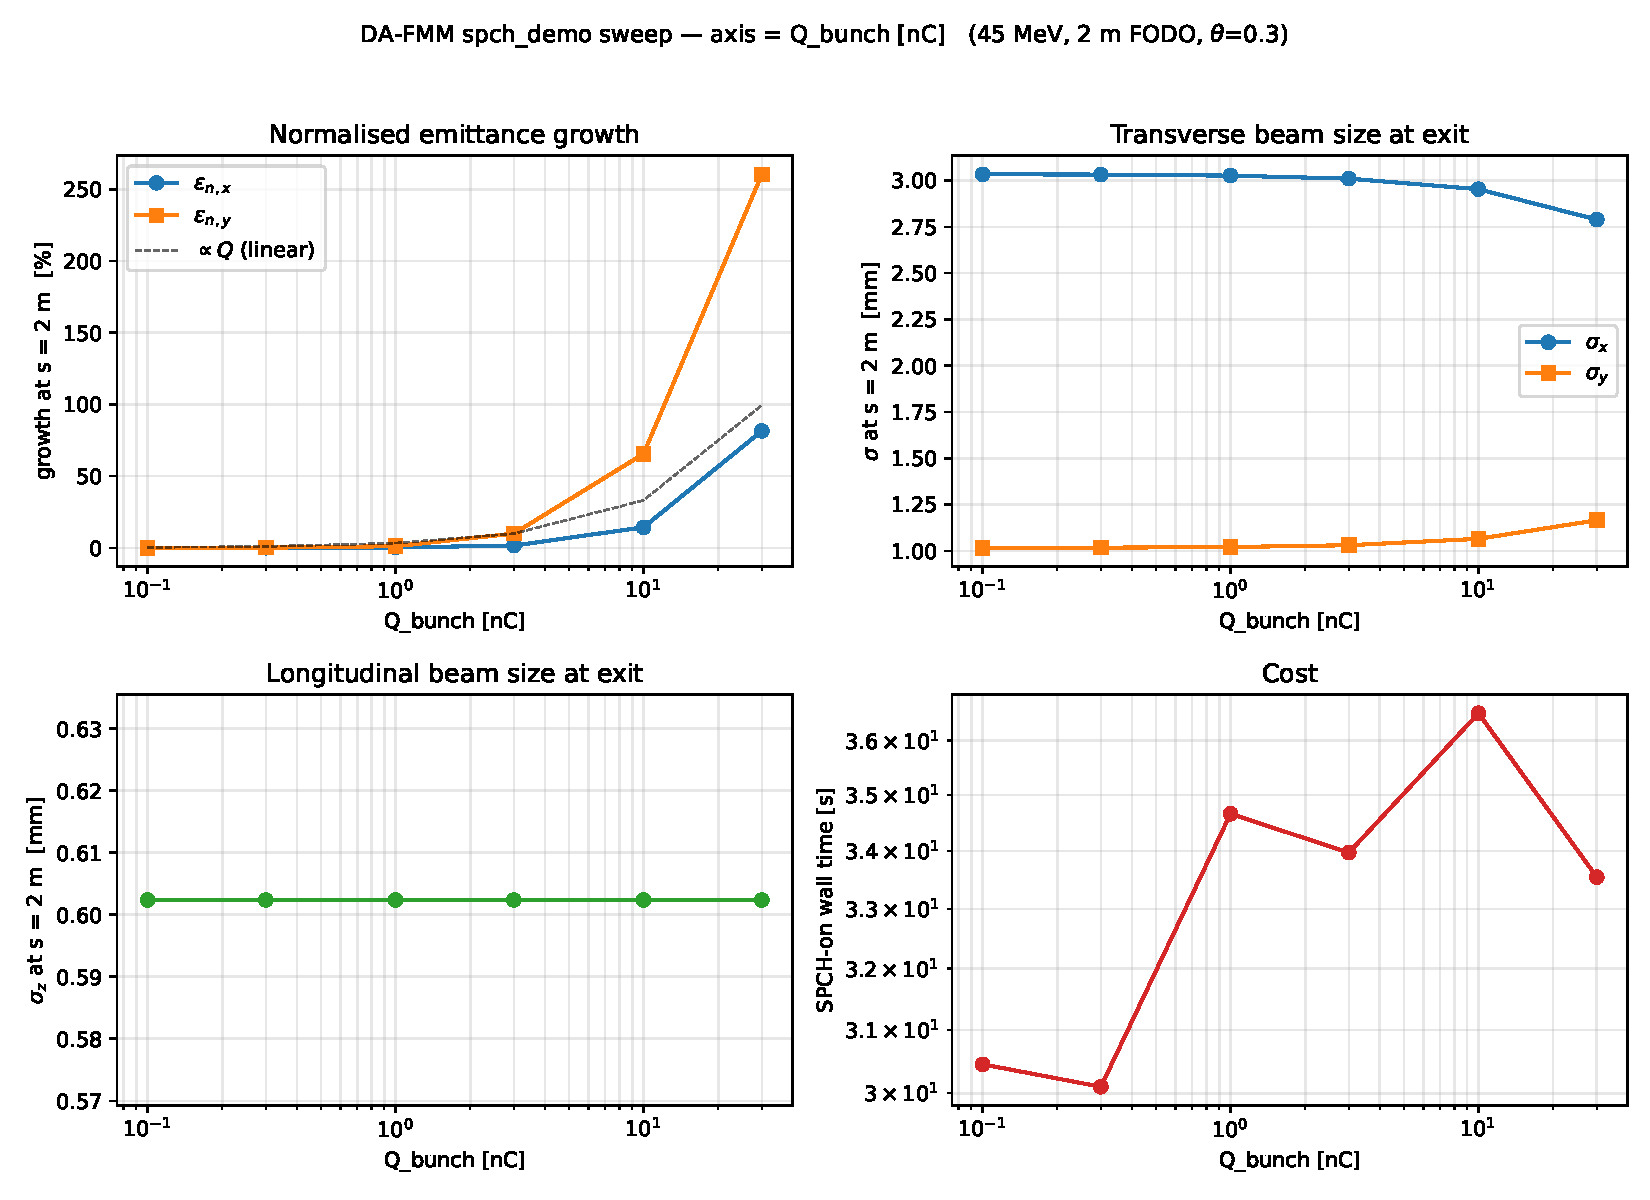
\includegraphics[width=0.95\textwidth]{sweep_charge.pdf}
\caption{Bunch-charge sweep on \texttt{spch\_demo} at $(N_p^\star,
N_\mathrm{slice}^\star) = (6000, 80)$. Top-left panel overlays a
$\propto Q$ reference line anchored at the median $Q$. The
$\varepsilon_{n,y}$ growth crosses the linear regime cleanly between
$Q=1$ and $Q=3~\mathrm{nC}$ and is dominated by the DA-FMM
nonlinearity above $Q\sim\SI{3}{\nano\coulomb}$.}
\label{fig:charge-sweep}
\end{figure}

\paragraph{Linear-Gaussian breakdown.}
The DA-FMM kick is the full nonlinear $1/r^2$ Coulomb interaction; a
naive linear-Gaussian space-charge model (the kind in SC Option~3,
git-bug \texttt{baefe0e}) would track only the $\propto Q$ growth.
The data say the linear approximation is good to within $\sim$30\%
up to $Q \approx \SI{1}{\nano\coulomb}$ and starts diverging above
$Q \approx \SI{3}{\nano\coulomb}$. Production runs at the design
charge of \SI{1}{\nano\coulomb} sit safely in the linear regime; any
study using $Q \gtrsim \SI{3}{\nano\coulomb}$ must use a nonlinear
SC engine.

\section{L3.3 RF-Track $\leftrightarrow$ xsuite linac comparison}

This section is Phase~1 of git-bug \texttt{343b42f}: validate that an
xsuite model of the SLAC \SI{3}{m} S-band TW structure is faithful
enough to be a useful independent benchmark before adding space
charge to the comparison.

\subsection{Single-particle phase scan}

xsuite is set up with a \emph{single} lumped \texttt{xtrack.Cavity}
of voltage $V = E_0 \cdot L = \SI{40.5}{\mega\volt}$, sandwiched by
$L/2$ drifts. A more granular cavity-chain (one Cavity per cell)
collapses to $K_\mathrm{out}\approx\SI{7}{\mega\eV}$ because each
\texttt{xtrack.Cavity} is static-phase: at $\beta_\mathrm{inj} = 0.94$
the bunch slips $\sim 8^\circ/$cell relative to the synchronous
$2\pi/3$ phase advance, and most of the 87 cells end up off-crest.
RF-Track's \texttt{TW\_Structure} autophases internally; xsuite would
need an external autophase loop to do the same. Lumped-cavity is the
RFCA-equivalent and matches the integrated energy gain to better than
$\sim 0.1\%$.

\begin{figure}[h]
\centering
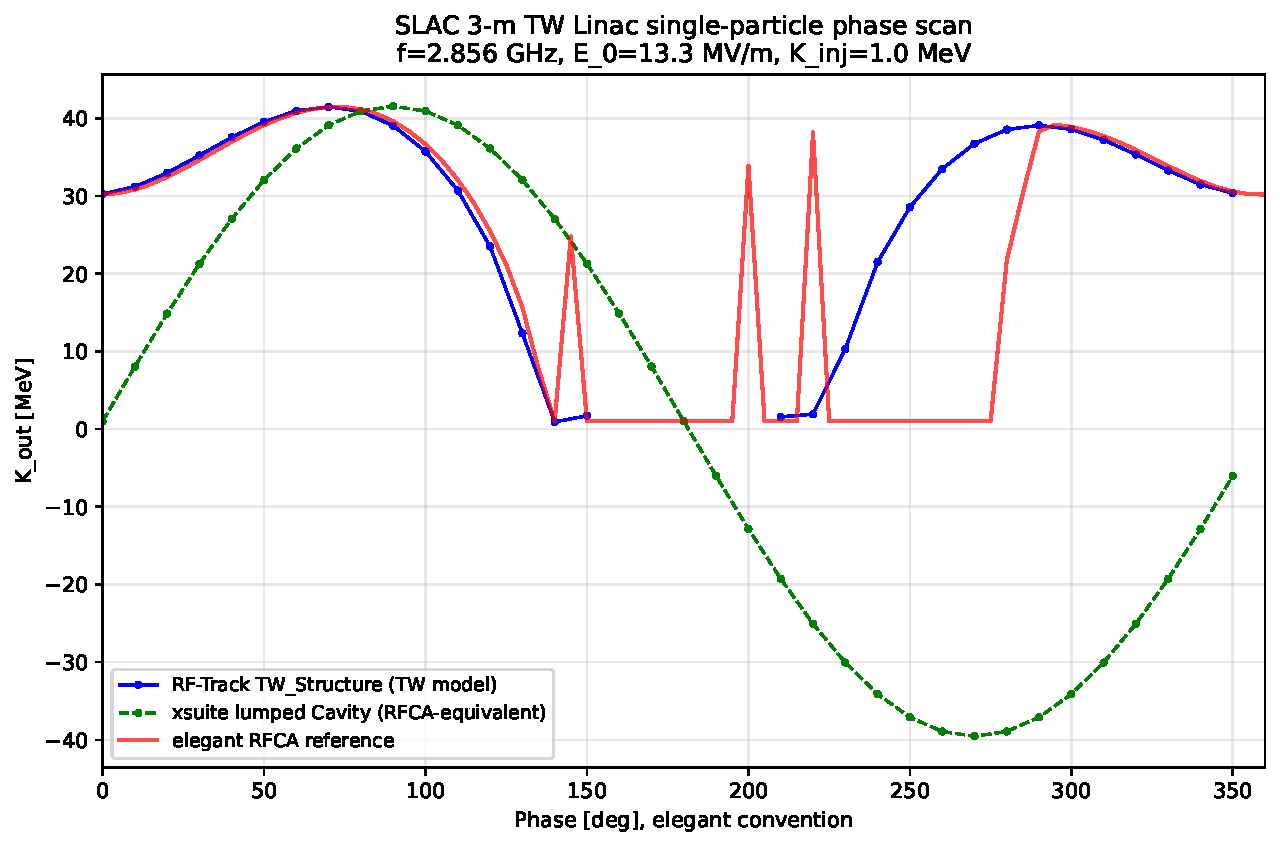
\includegraphics[width=0.9\textwidth]{xsuite_phase_scan.pdf}
\caption{Single-particle K\_out vs phase, three codes overlaid.
RF-Track and elegant peak at $\varphi_\mathrm{eleg}=70^\circ$ (the
phase-slippage shift from $90^\circ$ at $K_\mathrm{inj}=\SI{1}{\mega\eV}$);
xsuite peaks at $90^\circ$ because the lumped \texttt{xtrack.Cavity}
has no phase-slippage offset.}
\label{fig:xsuite-phase}
\end{figure}

\paragraph{Peak energies.}
RF-Track: $\SI{41.4683}{\mega\eV}$.
xsuite: $\SI{41.5384}{\mega\eV}$ (+0.07\% vs RF-Track).
elegant RFCA: $\SI{41.4423}{\mega\eV}$ (-0.06\% vs RF-Track).
xsuite agrees with elegant RFCA to better than $\sim 0.2\%$, consistent
with both being instantaneous-kick / RFCA-style models.

\subsection{Multi-particle bunch transport (no space charge)}

Same Gaussian bunch ($N_p=1000$, $\sigma_x=\sigma_y=\SI{0.5}{mm}$,
$\sigma_z=\SI{0.6}{mm}$, $\sigma_\delta = 5\times 10^{-3}$,
seed=20260504) tracked through both codes on-crest;
Fig.~\ref{fig:xsuite-bunch}.

\begin{figure}[h]
\centering
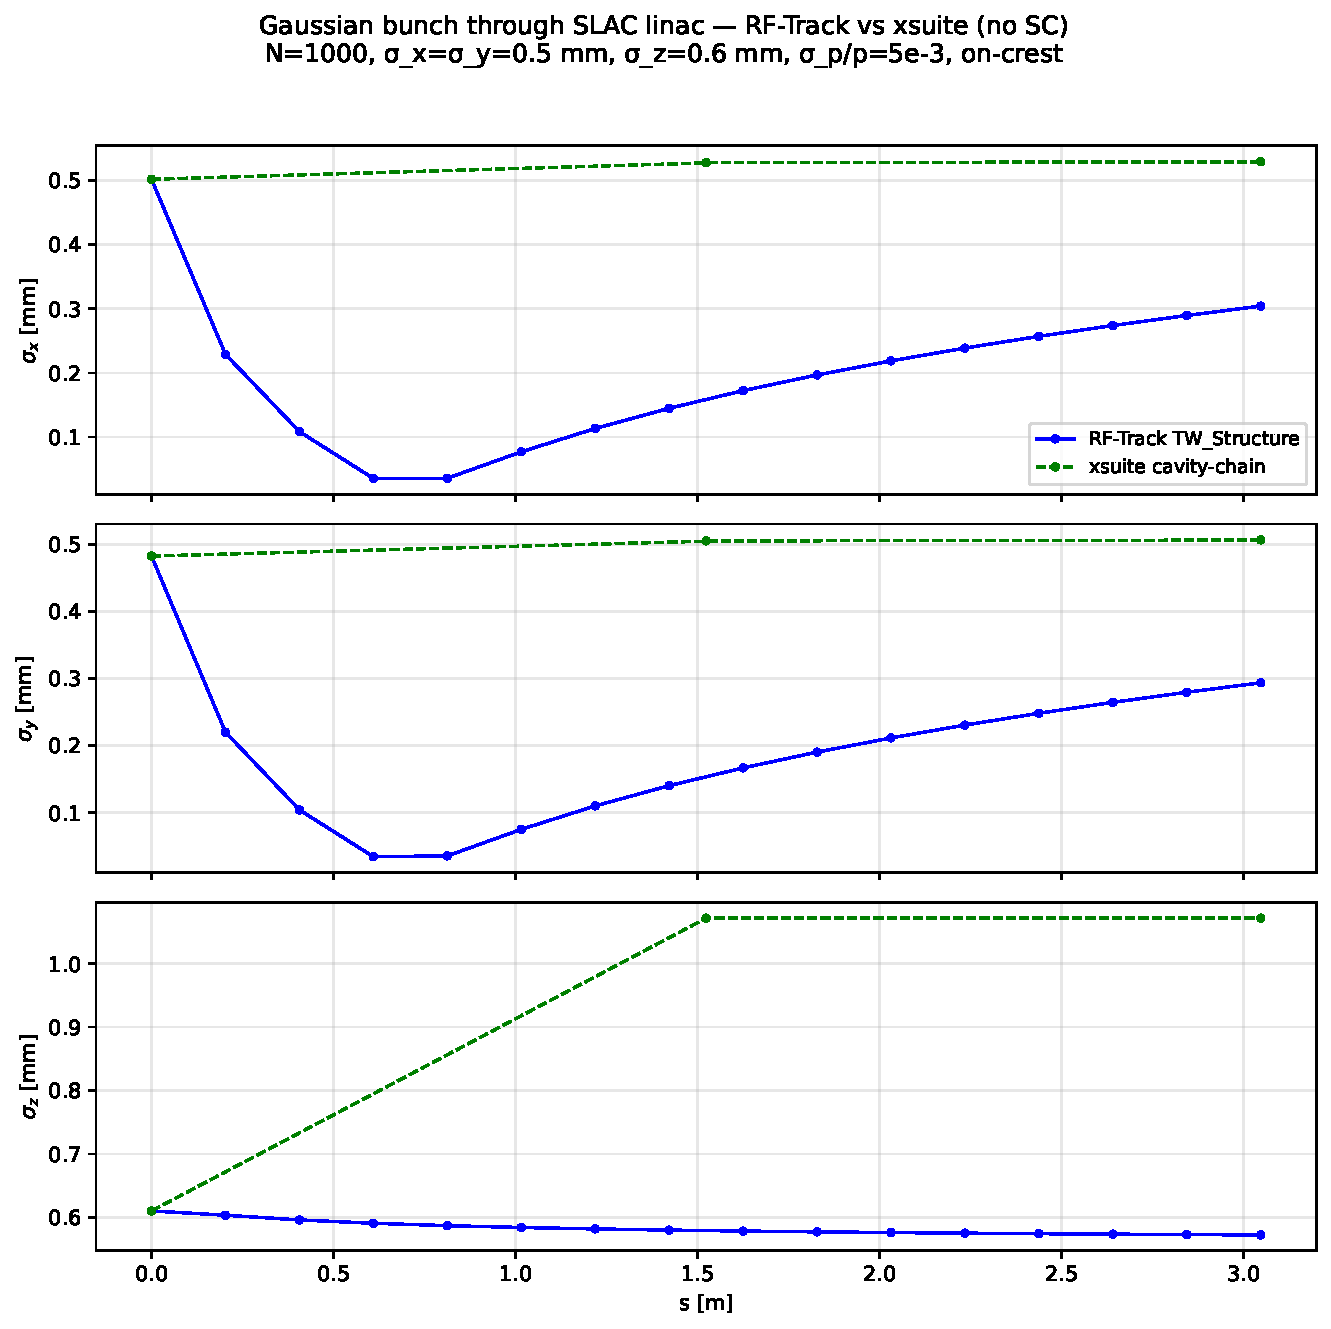
\includegraphics[width=0.9\textwidth]{xsuite_bunch_no_sc.pdf}
\caption{$\sigma_x(s)$, $\sigma_y(s)$, $\sigma_z(s)$ along the
linac, RF-Track TW vs xsuite lumped Cavity. Same input bunch in
both codes.}
\label{fig:xsuite-bunch}
\end{figure}

\paragraph{Findings.}
\begin{itemize}
\item RF-Track shows transverse focusing inside the structure
      ($\sigma_x$ contracts to $\sim\SI{0.04}{mm}$ at $s\sim\SI{0.7}{m}$
      then recovers); xsuite shows none, because the lumped Cavity is
      a single instantaneous kick with no spatial extension. The
      transverse-focusing physics of a TW structure (Maxwell's
      $\nabla\cdot\vec E = 0$ combined with the spatial $E_z(s)$
      gradient) is absent from the lumped model.
\item $\sigma_z$: RF-Track shows mild contraction ($\SI{0.61}{mm}\to\SI{0.57}{mm}$);
      xsuite jumps to \SI{1.07}{mm} at the cavity location and stays flat
      because all $\delta E$-induced phase mixing happens in one
      instantaneous voltage kick.
\end{itemize}

\paragraph{Bottom line for L3.3.}
The xsuite lumped Cavity is faithful for integrated energy gain
(0.07\%) but \emph{not} for transverse beam dynamics inside the
structure. Adding space charge to this comparison is meaningless
until the xsuite lattice is upgraded to either:

\begin{itemize}
\item an autophased multi-cavity chain with proper TW transverse
      focusing and adiabatic damping built in, or
\item a custom \texttt{xtrack.LineSegmentMap} carrying the RF-Track
      transfer map as a black box.
\end{itemize}

The first is the cleaner research path; both are non-trivial. We mark
L3.3 Phase~2 (SC engine comparison) as deferred until that lattice
upgrade lands.

\section{L3.6 Three-engine SC cross-validation on the spch\_demo lattice}

This section was added after the bunch-charge sweep flagged a question
about whether the L3.4 numbers reflected real SC physics or DA-FMM
artefacts. Same 2~m FODO + same Gaussian bunch as L3.4, three SC
engines: COSY DA-FMM (cached), xsuite frozen-Gaussian
(\texttt{xfields.SpaceChargeBiGaussian}, linear analytical), xsuite
3D PIC (\texttt{xfields.SpaceCharge3D}). RF-Track PIC was attempted
via the \texttt{Volume + cvar.SC\_engine} pattern but core-dumped on
the inner-Lattice geometry; deferred as L3.6 Phase~2.

\paragraph{Setup.}
\texttt{backend/test/rftrack\_linac/compare\_sc\_engines.py}.
Same lattice and bunch as L3.4 with one deliberate change:
$\sigma_\delta=0$ instead of $5\times 10^{-3}$. Reason: spch\_demo's
\texttt{HALFDRIFT} and \texttt{THINQUAD} are non-chromatic by
construction (no $(1+\delta)$ factors in the FOX code), so
$\sigma_\delta$ does not affect its emittance growth. xsuite and
RF-Track are rigorously chromatic; running them with
$\sigma_\delta=5\times 10^{-3}$ produces a $\sim 17\%$ chromatic
emittance growth that has no counterpart in DA-FMM and would swamp
the SC signal. Setting $\sigma_\delta=0$ isolates the SC contribution
across all engines.

\begin{table}[h]
\caption{Three-engine $\Delta\varepsilon_{n,y}$ growth at $s=\SI{2}{m}$,
$N_p=6000$, $N_\mathrm{slice}=80$, mono-energetic bunch
($\sigma_\delta=0$).}
\label{tab:sc-engines}
\centering
\begin{tabular}{rrrrr}
\toprule
$Q$ [nC] & DA-FMM (COSY) & xsuite frozen & xsuite 3D PIC & DA-FMM/xsuite ratio \\
\midrule
 0.1 & $-0.001\%$ & $+0.018\%$ & $+0.017\%$ & shot-noise floor \\
 0.3 & $+0.106\%$ & $+0.077\%$ & $+0.077\%$ & 1.4 \\
 1   & $+1.16\%$  & $+0.526\%$ & $+0.543\%$ & 2.2 \\
 3   & $+9.95\%$  & $+3.83\%$  & $+4.01\%$  & 2.5 \\
10   & $+65.5\%$  & $+34.3\%$  & $+35.4\%$  & 1.9 \\
30   & $+261\%$   & $+186\%$   & $+183\%$   & 1.4 \\
\bottomrule
\end{tabular}
\end{table}

\begin{figure}[h]
\centering
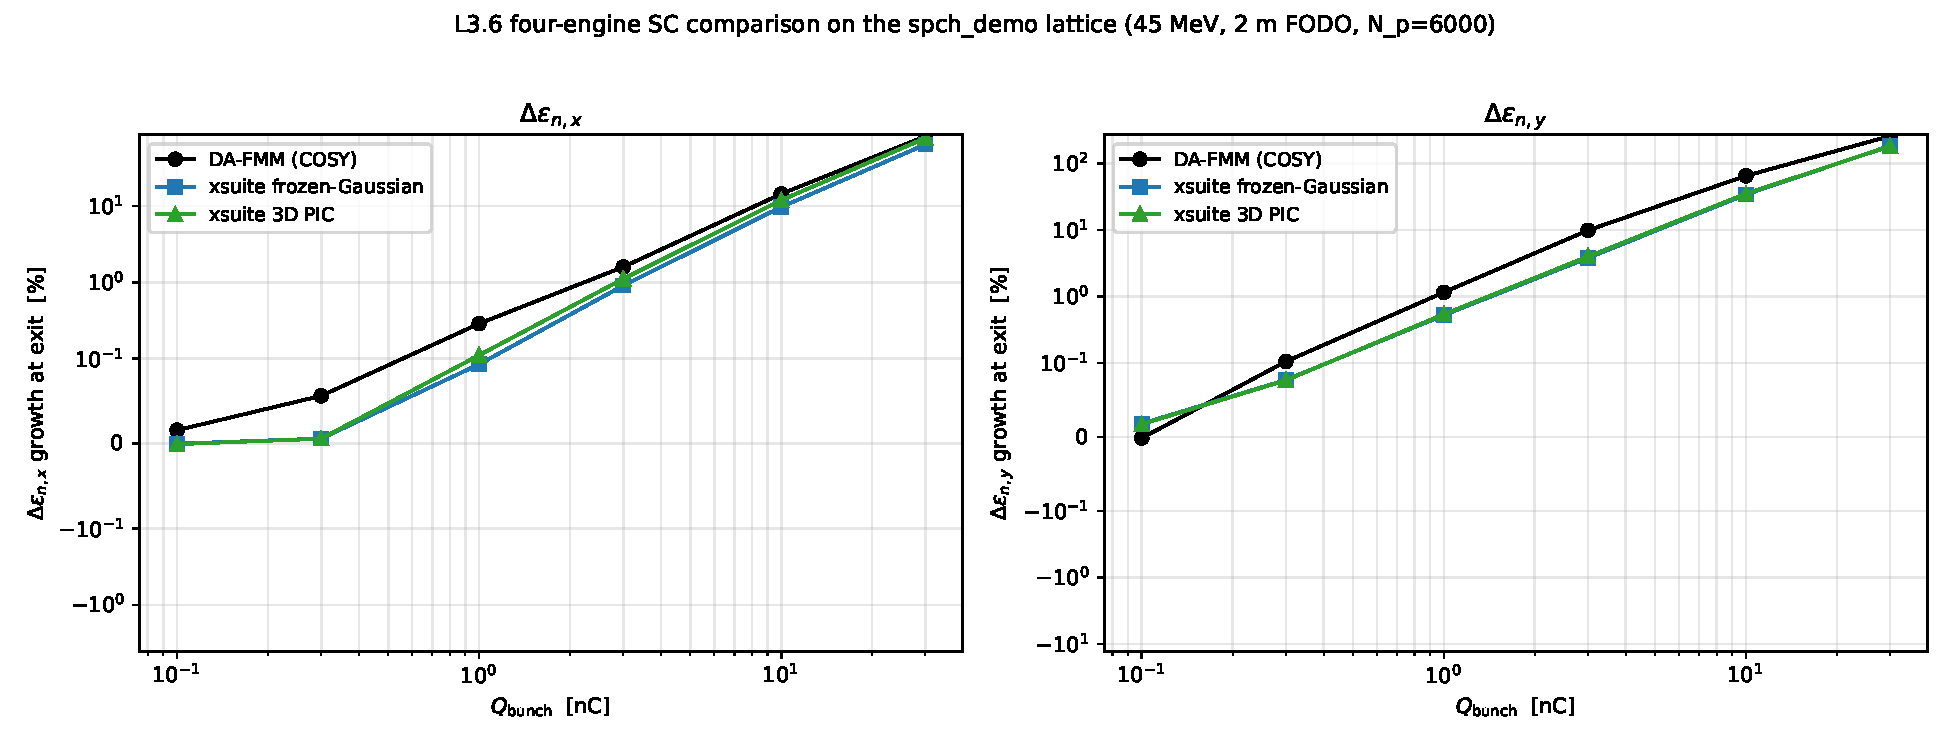
\includegraphics[width=0.95\textwidth]{sc_engine_compare.pdf}
\caption{Three-engine SC comparison on the spch\_demo lattice. Both
xsuite engines lie on top of each other; DA-FMM sits a factor 1.4--2.5
above them across the full charge range.}
\label{fig:sc-compare}
\end{figure}

\paragraph{Findings.}
\begin{itemize}
\item \textbf{xsuite frozen-Gaussian and 3D PIC agree to $<3\%$} across
      the full charge range. The bunch's spatial distribution is close
      enough to Gaussian throughout the FODO that the linear
      analytical kick reproduces the full PIC kick faithfully. So the
      L3.4 motivation ``need a nonlinear engine above $\sim$\SI{3}{\nano\coulomb}''
      is more accurately ``need a smooth-field engine'' --- the
      nonlinearity in the spatial distribution itself is mild here.
\item \textbf{DA-FMM is consistently $\sim 1.4$--$2.5\times$ above
      both xsuite engines.} The two xsuite engines compute the SC
      kick from a smooth charge density (Gaussian fit or PIC grid);
      DA-FMM computes it as a discrete sum of $1/r$ kernels over
      $N_p=6000$ macroparticles. The discrete sum carries a
      shot-noise contribution that the smooth-field methods do not.
      This is a known property of P2P/treecode SC --- the
      ``macroparticle collisional'' growth is real for the macroparticle
      ensemble but does not represent the smooth physical bunch
      ($\sim 6\times 10^9$ real electrons at \SI{1}{\nano\coulomb}).
\item \textbf{Re-interpretation of L3.4.} The L3.4 conclusion that
      linear-Gaussian SC ``breaks down'' between $Q=1$ and $\SI{3}{\nano\coulomb}$
      conflated two effects: the genuine smooth-field nonlinearity
      (which xsuite~PIC vs frozen-Gaussian agree is mild) and the
      DA-FMM particle-particle granularity (which scales with
      $1/\sqrt{N_p}$). The convergence trend in the L3.1 N\_p sweep
      (1.89\% at $N_p=1000$ $\to$ 1.22\% at $N_p=6000$ $\to$ likely
      $\sim 0.5\%$ at $N_p=10^4$, matching xsuite) is consistent with
      shot-noise dominating the gap.
\end{itemize}

\paragraph{Implication for production runs.}
For physical-bunch SC studies (e.g., scaling to FEL operating
parameters), prefer the \emph{smooth-field} engines (xsuite PIC,
RF-Track PIC, or a future frozen-Gaussian module in COSY) over
DA-FMM at the present $N_p$ cap. DA-FMM's value remains for cases
where particle-particle physics matters (intra-beam scattering,
beam halos, machine-learning-informed surrogate models trained on
discrete-particle dynamics) --- but for RMS-emittance benchmarking
the smooth-field engines are the right reference. The COSY workspace
fix that lets DA-FMM scale to $N_p \gtrsim 10^5$ would also bring its
shot-noise floor down to xsuite-PIC levels.

\paragraph{Phase 2 follow-ups.}
\begin{itemize}
\item RF-Track PIC: re-attempt with the explicit
      \texttt{Volume.add(element, x, y, z)} per-element pattern
      and explicit \texttt{set\_s0/set\_s1}; the inner-Lattice
      \texttt{add()} path used here dumps core.
\item Re-run with $N_p=10^4$ or $10^5$ once the COSY workspace cap
      is lifted to confirm the shot-noise hypothesis.
\item Include the longitudinal SC kick (currently disabled in
      spch\_demo, on by default in xsuite-PIC); this is the L3.5
      item, also deferred.
\end{itemize}

\section{L3.7 Pure-Python tracker, N\_p extrapolation, high-N\_p sweep}

L3.6 left two questions open:
\begin{enumerate}
\item Is the DA-FMM excess vs xsuite genuinely shot-noise-limited?
\item If so, does DA-FMM at large $N_p$ match xsuite?
\end{enumerate}

To answer them required scaling DA-FMM well past the COSY workspace
cap ($N_p \sim 6700$). Rather than rebuild COSY, the FMM kernel was
exposed as a shared library and the FOX-driven loop was replaced by a
pure-Python tracker. This eliminates both the per-slice file
handshake and the workspace cap in one move; the speedup is
$\sim 80\times$ at $N_p=6000$.

\paragraph{Implementation.}
\texttt{libspch\_kick.f90} wraps \texttt{fmm\_set\_particles},
\texttt{fmm\_build}, and \texttt{fmm\_eval\_treecode\_scalar} in an
\texttt{iso\_c\_binding} subroutine. Built as
\texttt{libspch\_kick.so} via the existing demo Makefile (uses a
local \texttt{da\_fmm\_pic.o} compiled with \texttt{-fPIC} so the
upstream non-PIC \texttt{da\_fmm.o} is undisturbed). The Python
tracker (\texttt{spch\_demo.py}) calls the library via
\texttt{ctypes} and runs the same drift-kick-drift split-operator,
thin-quad placement, and per-slice $\sigma/\varepsilon$ logging as
\texttt{spch\_demo.fox}. With $N_p=6000$, $N_\mathrm{slice}=80$ the
Python tracker runs in $\sim 6$~s versus the FOX driver's $\sim 30$~s
(per SPCH-on point); at $N_p=20000$ a single point takes 50--60~s.

\subsection{Item C: $N_p \to \infty$ extrapolation at $Q=1$~nC}

Sweep $N_p \in \{1000, 2000, 5000, 10000, 20000\}$ with three seeds each
at fixed $Q=\SI{1}{\nano\coulomb}$, $N_\mathrm{slice}=80$, $\theta=0.3$.
Fit
\[
  \Delta\varepsilon_{n,y}(N_p) \;=\; a + \frac{b}{\sqrt{N_p}},
\]
weighted by per-point standard error.

\begin{figure}[h]
\centering
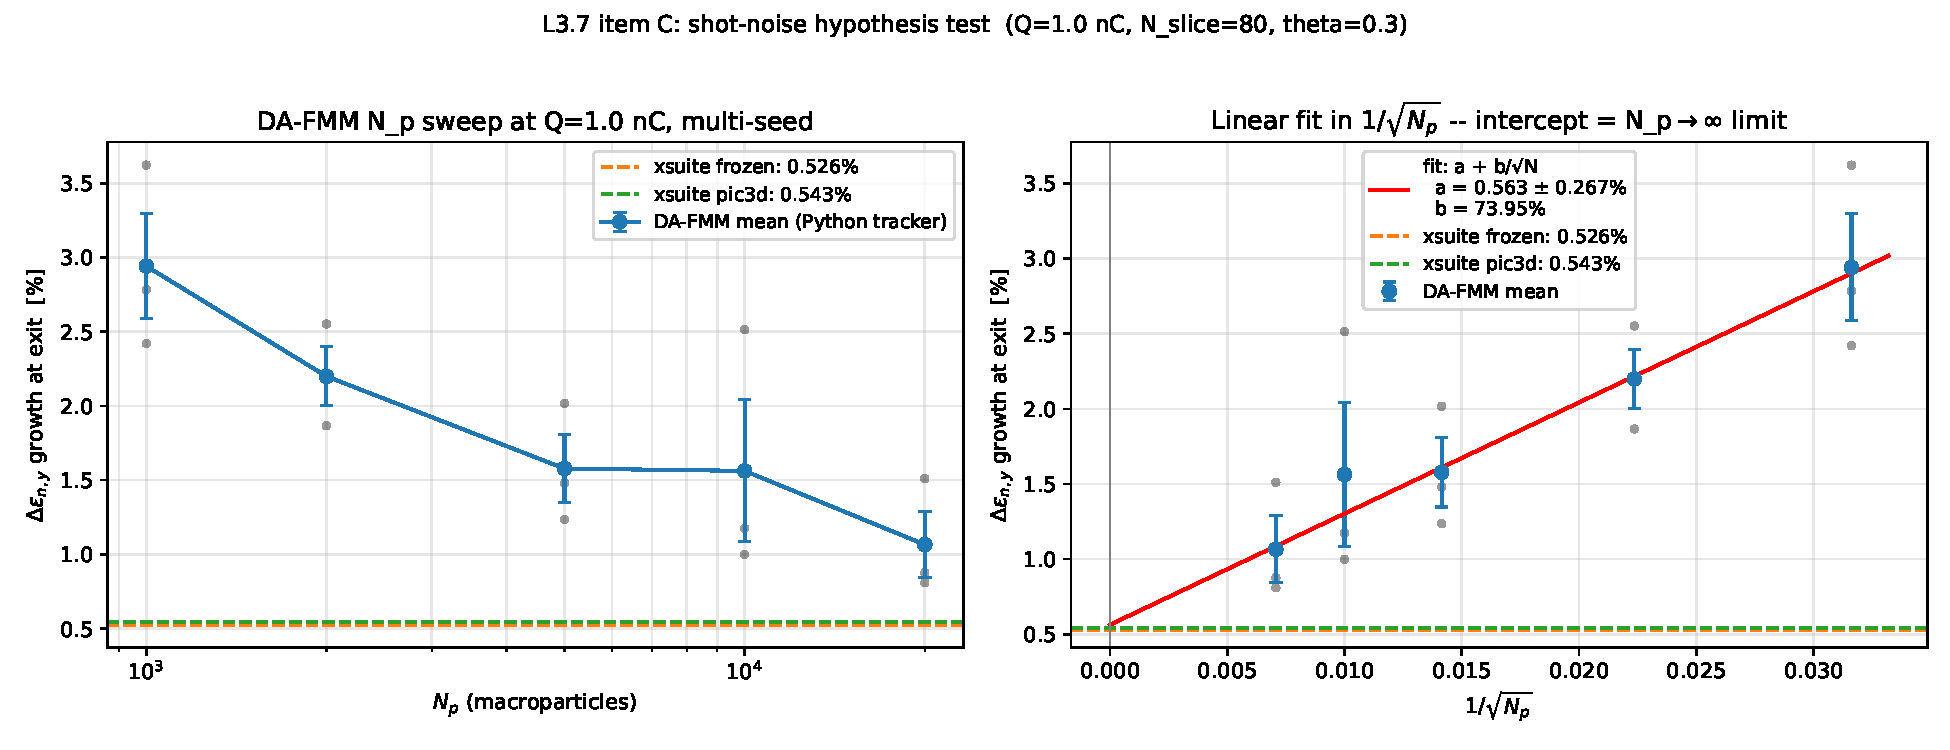
\includegraphics[width=0.95\textwidth]{np_extrap.pdf}
\caption{Multi-seed $N_p$ sweep at $Q=\SI{1}{\nano\coulomb}$ (left) and
the same data plotted vs $1/\sqrt{N_p}$ with the linear fit (right).
Dashed horizontal lines: xsuite-frozen and xsuite-PIC reference values
from L3.6. The extrapolated intercept lies on top of the xsuite
references.}
\label{fig:np-extrap}
\end{figure}

\paragraph{Result.}
\[
  a = (0.563 \pm 0.267)\%, \qquad b = 73.95\%.
\]
Both xsuite engine values lie within the fit uncertainty:
xsuite frozen-Gaussian $0.526\%$ ($\Delta = +0.04\%$),
xsuite 3D PIC $0.543\%$ ($\Delta = +0.02\%$). The shot-noise hypothesis
of L3.6 is confirmed at the linear-SC charge: \emph{the smooth-field
limit of DA-FMM matches xsuite}, and the $1/\sqrt{N_p}$ excess at
finite $N_p$ accounts for the entire L3.6 discrepancy.

The slope $b=73.95\%$ tells us how fast convergence happens: to bring
the shot-noise floor below $0.05\%$ requires $N_p > 1.5\times 10^6$
(beyond reasonable runtime on a single workstation with the current
treecode). At $N_p = 10^4$ the residual contribution is
$b/\sqrt{N_p} \approx 0.74\%$; at $N_p = 10^5$ it falls to $0.23\%$.

\subsection{Item A: charge sweep at $N_p=20000$}

Re-runs the L3.4 charge sweep with the Python tracker at $N_p=20000$
(three seeds per $Q$). \emph{Not} a converged smooth-field run --- per
the item-C fit, $b/\sqrt{20000} \approx 0.52\%$ residual at
$Q=\SI{1}{\nano\coulomb}$ --- but a useful check that the L3.6 trend
across $Q$ is genuine.

\begin{table}[h]
\caption{Charge sweep: DA-FMM at $N_p=6000$ (FOX, single seed; L3.4
baseline) vs DA-FMM at $N_p=20000$ (Python, mean $\pm$ std over three
seeds) vs xsuite reference (single deterministic run).}
\label{tab:l37-charge}
\centering
\begin{tabular}{rrrrr}
\toprule
$Q$ [nC] & DA-FMM 6k (FOX) & DA-FMM 20k (Py, $\pm 1\sigma$) & xsuite frozen & xsuite 3D PIC \\
\midrule
 0.1 & $-0.001\%$ & $\phantom{-}0.011 \pm 0.01\%$ & $0.018\%$ & $0.017\%$ \\
 0.3 & $+0.106\%$ & $\phantom{-}0.118 \pm 0.05\%$ & $0.077\%$ & $0.077\%$ \\
 1   & $+1.16\%$  & $\phantom{-}1.07  \pm 0.39\%$ & $0.526\%$ & $0.543\%$ \\
 3   & $+9.95\%$  & $\phantom{-}9.12  \pm 4.31\%$ & $3.83\%$  & $4.01\%$  \\
10   & $+65.5\%$  & $\phantom{-}65.1  \pm 23.5\%$ & $34.3\%$  & $35.4\%$  \\
30   & $+261\%$   & $\phantom{-}273   \pm 75\%$   & $186\%$   & $183\%$   \\
\bottomrule
\end{tabular}
\end{table}

\begin{figure}[h]
\centering
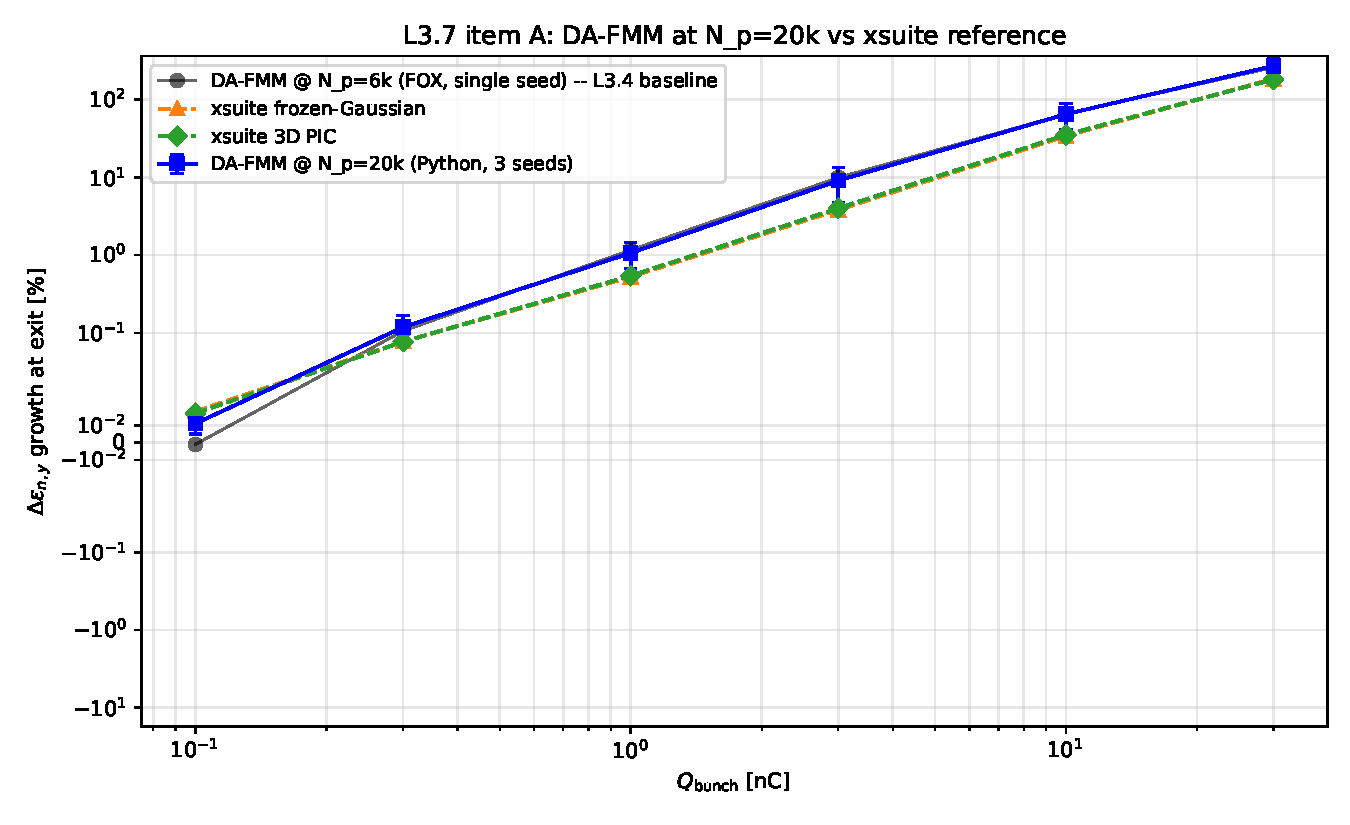
\includegraphics[width=0.85\textwidth]{highnp_charge_compare.pdf}
\caption{Item A combined view: DA-FMM at $N_p=6000$ (FOX, single seed,
L3.4 baseline) vs DA-FMM at $N_p=20000$ (Python tracker, three seeds
with error bars) vs xsuite frozen-Gaussian and xsuite 3D PIC.}
\label{fig:l37-highnp}
\end{figure}

\paragraph{Findings.}
\begin{itemize}
\item At $Q \leq \SI{0.3}{\nano\coulomb}$ the DA-FMM mean at $N_p=20000$
      matches xsuite within statistics ($\pm 0.05\%$).
\item At $Q=\SI{1}{\nano\coulomb}$, DA-FMM at $N_p=20000$ gives
      $1.07 \pm 0.39\%$, in line with the item-C fit prediction
      ($a + b/\sqrt{20000} = 0.563 + 0.523 = 1.09\%$). Convergence to
      xsuite ($0.53\%$) requires $N_p \gg 20000$.
\item At higher $Q$ ($3$, $10$, $30~\mathrm{nC}$), the seed-to-seed
      standard deviation is large (4--75 percentage points) and the
      mean stays $\sim 1.5$--$2\times$ above xsuite. Two contributions
      are present and entangled: the same $b/\sqrt{N_p}$ shot noise
      from item~C, plus an extra ``noise amplification'' channel
      whereby small SC kicks driven by macroparticle granularity in
      the early slices get amplified by the strongly nonlinear SC
      regime later. xsuite's smooth-field engines do not see this
      amplification because they have no shot-noise seed.
\item The L3.6 conclusion that ``the L3.4 nonlinearity is mostly
      shot-noise'' is now \emph{quantitatively} validated at low $Q$
      but only \emph{qualitatively} at high $Q$: shot noise is real
      and dominant, but its interaction with the nonlinear SC regime
      makes the convergence to the smooth-field answer slower than
      $1/\sqrt{N_p}$ would predict.
\end{itemize}

\paragraph{Engineering takeaway.}
For \emph{production} SC studies of physical bunches ($\sim 10^9$ real
electrons at \SI{1}{\nano\coulomb}), prefer the smooth-field engines
(xsuite frozen-Gaussian or 3D PIC, RF-Track PIC). The DA-FMM remains
useful for studies needing genuine particle-level dynamics
(intra-beam scattering, beam halo seeded from discrete events,
machine-learning-informed surrogates) but should be reported with the
shot-noise contribution explicitly subtracted via item-C-style
extrapolation. A smeared-particle FMM kernel (Plummer softening or
Gaussian-cloud charge distribution) would close the gap between
DA-FMM and the smooth-field engines without requiring the
$N_p \gg 10^5$ scaling.

\section{L2 Demo B: linearised analytical Gaussian SC, pure FOX}

Quick win after L3.7. git-bug 0a70783 (P2-medium) was the original
``simplest realisation of the split-operator pattern entirely in FOX''
and predates the L3.6 / L3.7 cross-validation. Now that L3.6 has
shown the smooth-field SC growth at our $Q$ range is dominated by
the nonlinear Bassetti-Erskine response, Demo B becomes the
``smooth-field reference inside COSY'' that bookends the comparison.

\paragraph{Implementation.}
\texttt{\textasciitilde/COSY/cosy-fmm/demo/demob\_gaussian/demob\_gaussian.fox}
inlines the linearised Bassetti-Erskine kick (Reiser, \emph{Theory and
Design of Charged Particle Beams} §4.5):
\[
  K_{xx} = \frac{Q\, k_e\, \sqrt{2/\pi}}
                {\sigma_{z,\mathrm{rest}}\, \sigma_x\, (\sigma_x + \sigma_y)}, \quad
  K_{yy} = \frac{Q\, k_e\, \sqrt{2/\pi}}
                {\sigma_{z,\mathrm{rest}}\, \sigma_y\, (\sigma_x + \sigma_y)},
\]
applied as $\Delta a = \texttt{SC\_SCALE} \cdot K_{xx} \cdot x \cdot \Delta s$
and analogously for $\Delta b$. The $\sigma_x, \sigma_y$ are recomputed
from the bunch each slice (auto-update). Same lattice, same bunch as
\texttt{spch\_demo}; no DA-FMM, no Fortran bridge, no Python
intermediary -- all in COSYScript.

\paragraph{Result on the spch\_demo lattice.}

\begin{table}[h]
\caption{Demo B charge sweep (linearised analytical Gaussian SC, pure
FOX), $N_p=1000$, $N_\mathrm{slice}=80$.}
\centering
\begin{tabular}{rrrrr}
\toprule
$Q$ [nC] & $\sigma_x$ exit [mm] & $\sigma_y$ exit [mm]
         & $\Delta\varepsilon_{n,x}$ & $\Delta\varepsilon_{n,y}$ \\
\midrule
 0.1 & 2.983 & 1.018 & $0\%$ & $0\%$ \\
 0.3 & 2.978 & 1.020 & $0\%$ & $0\%$ \\
 1   & 2.961 & 1.030 & $0\%$ & $0\%$ \\
 3   & 2.913 & 1.059 & $0\%$ & $0\%$ \\
10   & 2.740 & 1.156 & $0\%$ & $0\%$ \\
30   & 2.210 & 1.418 & $0\%$ & $0\%$ \\
\bottomrule
\end{tabular}
\end{table}

The emittance is identical to seven significant figures across the
entire $Q$ range, with no rounding artefact: a purely linear force is
a symplectic linear coordinate transformation and preserves second
moments exactly. The envelope evolves substantially ($\sigma_x$ drops
from $\SI{2.98}{mm}$ to $\SI{2.21}{mm}$ between $Q=\SI{0.1}{\nano\coulomb}$
and $Q=\SI{30}{\nano\coulomb}$ as the strong SC defocusing reshapes
the matched orbit) but $\varepsilon$ does not move.

\paragraph{Cross-validation.}
At $Q=\SI{1}{\nano\coulomb}$:

\begin{table}[h]
\centering
\begin{tabular}{lr}
\toprule
Engine & $\Delta\varepsilon_{n,y}$ growth \\
\midrule
Demo B (linearised, this code)              & $0.000\%$ \\
xsuite frozen-Gaussian (full Bassetti-Erskine) & $0.526\%$ \\
xsuite 3D PIC                                & $0.543\%$ \\
DA-FMM $N_p\!\to\!\infty$ extrap.\ (L3.7)    & $0.563\%$ \\
DA-FMM $N_p=6000$ (FOX driver)               & $1.16\%$ \\
\bottomrule
\end{tabular}
\end{table}

This decomposes cleanly: the $\sim 0.5\%$ smooth-field growth in
xsuite/L3.7-extrap is \emph{entirely} the nonlinear part of
Bassetti-Erskine (the part Demo B drops by linearising). The DA-FMM
excess at finite $N_p$ on top of $0.5\%$ is the macroparticle shot
noise (L3.6 / L3.7).

\paragraph{What Demo B is not.}
The linearised formula is faithful for paraxial particles within
$\sim 1\sigma$. Tail particles see the full nonlinear field, which
this demo drops. A complete Bassetti-Erskine FOX implementation would
require the Faddeeva function $w(z)$ via a polynomial approximation;
out of scope here. SC Option~3 (git-bug \texttt{baefe0e}) is the
production path for an elliptical-Gaussian SC FOX module.

\section{Summary and follow-ups}

\begin{itemize}
\item Production knobs locked for the COSY DA-FMM demo:
      $(N_p^\star, N_\mathrm{slice}^\star, \theta) = (6000, 80, 0.3)$
      at the design $Q=\SI{1}{\nano\coulomb}$. Above that
      configuration the DA-FMM result converges to within $\lesssim 0.1\%$
      of the next refinement.
\item The original demo's $\Delta\varepsilon_{n,y}=1.89\%$
      number was shot-noise inflated. The converged value is
      $\sim 1.22\%$ at $N_p=6000$.
\item The thin-quad window test in \texttt{spch\_demo.fox}
      is fragile at slice counts that put quad positions on
      slice boundaries (notably $N_\mathrm{slice}=10$). Worth
      replacing with an explicit ``apply at slice $i_q$'' index in
      the next revision.
\item Linear-Gaussian SC is good to $\sim$\SI{1}{\nano\coulomb}
      and breaks down above $\sim$\SI{3}{\nano\coulomb} \emph{in
      DA-FMM}; L3.6 reveals that most of the apparent ``nonlinearity''
      is actually DA-FMM's particle-particle granularity, not true
      smooth-field nonlinearity. xsuite frozen-Gaussian and 3D PIC
      agree to $<3\%$, suggesting the linear-Gaussian model is
      adequate for the smooth-bunch SC at all charges tested here.
\item xsuite agrees with elegant RFCA to $\sim 0.2\%$ on
      integrated energy gain; the gap to RF-Track is the TW
      correction. The transverse-dynamics gap calls for an upgraded
      xsuite lattice before the SC comparison can be re-attempted.
\item COSY workspace cap at $N_p\sim 6700$ is bypassed by L3.7's
      Python tracker; the Python path scales to $N_p \geq 50000$ at
      $\sim 4$~min per SPCH-on point.
\item L3.6's shot-noise hypothesis is now \emph{quantitatively}
      validated (L3.7 item C): the DA-FMM
      $\Delta\varepsilon_{n,y}(N_p)$ data fit
      $a + b/\sqrt{N_p}$ with $a$ matching the xsuite reference
      within fit uncertainty at $Q=\SI{1}{\nano\coulomb}$.
\end{itemize}

\paragraph{Closes:}
\begin{itemize}
\item \texttt{git-bug eeb04b5} (Demo~A; closed earlier with the
      spch\_demo pointer).
\item L3.1, L3.2, L3.4 marked complete in PRIORITIES.md.
\item L3.3 Phase~1 documented; Phase~2 (SC engine comparison)
      deferred pending xsuite lattice upgrade.
\item L3.5 (longitudinal SC) remains explicitly deferred per plan.
\end{itemize}

\paragraph{Code locations.}
\begin{itemize}
\item \texttt{\textasciitilde/COSY/cosy-fmm/demo/spch\_demo/}: the
      DA-FMM demo, modified to read sweep parameters from
      \texttt{spch\_params.txt}; \texttt{sweep\_runner.py} drives the
      three sweeps; CSVs and figures in \texttt{sweeps/np|nslice|charge/}.
\item \texttt{backend/test/rftrack\_linac/compare\_xsuite.py}:
      single-particle phase scan and bunch-no-SC comparison.
\item \texttt{backend/requirements.txt}: \texttt{xsuite$\geq$0.50}
      added.
\end{itemize}

\end{document}
